\documentclass{estilo}
\usepackage[spanish]{babel}
\usepackage{float}
\usepackage{amsfonts}       % para las negrita de pizarra
\usepackage{amssymb}        % para simbolos matematicos
\usepackage{multirow}       % para las tablas
\usepackage{siunitx}        % para unidades y formato numérico
\usepackage{dsfont}

% Paquetes configurables
\usepackage{amsthm}         % para teoremas, pruebas y definiciones
\newtheorem*{definicion}{Definición}
\usepackage{amsmath}        % para múltiples utilidades
%\newcommand*\diff{\mathop{}\!\mathrm{d}}
\usepackage{listings}       % para snippets con estilo personalizable
\usepackage{xcolor}
\definecolor{codegreen}{rgb}{0,0.6,0}
\definecolor{codegray}{rgb}{0.5,0.5,0.5}
\definecolor{codepurple}{rgb}{0.58,0,0.82}
\definecolor{backcolour}{rgb}{0.95,0.95,0.92}
\lstdefinestyle{mystyle}{
    backgroundcolor=\color{backcolour},
    commentstyle=\color{codegreen},
    keywordstyle=\color{magenta},
    numberstyle=\tiny\color{codegray},
    stringstyle=\color{codepurple},
    basicstyle=\ttfamily\footnotesize,
    breakatwhitespace=false,
    breaklines=true,
    captionpos=b,
    keepspaces=true,
    numbers=left,
    numbersep=5pt,
    showspaces=false,
    showstringspaces=false,
    showtabs=false,
    tabsize=2
}
\lstset{style=mystyle}
\usepackage{enumitem,multicol,setspace} % para las multicolumnas
\newcounter{subenum}[enumi]
\renewcommand{\thesubenum}{\arabic{subenum}}
\usepackage[nomessages]{fp}
\FPeval\thecolwidth{round(1/4:4)}% Specify number of columns -> column width
\newcommand{\newitem}[1]{%
    \refstepcounter{subenum}%
    \parbox{\dimexpr\thecolwidth\linewidth-.5\columnsep}{%
        \makebox[\labelwidth][r]{(\thesubenum)\hspace*{\labelsep}}%
        #1}\hfill%
}
\usepackage{scalerel,stackengine} % para el sombrero
\stackMath
\newcommand\rhat[1]{%
    \savestack{\tmpbox}{\stretchto{%
        \scaleto{%
            \scalerel*[\widthof{\ensuremath{#1}}]{\kern-.6pt\bigwedge\kern-.6pt}%
            {\rule[-\textheight/2]{1ex}{\textheight}}%WIDTH-LIMITED BIG WEDGE
        }{\textheight}% 
    }{0.5ex}}%
    \stackon[1pt]{#1}{\tmpbox}%
}
\parskip 1ex
\usepackage{mathtools}      % floor y ceil
\DeclarePairedDelimiter\ceil{\lceil}{\rceil}
\DeclarePairedDelimiter\floor{\lfloor}{\rfloor}
\usepackage[style=authoryear-comp]{biblatex}

\begin{document}
    \maketitle

    \newpage
    \tableofcontents
    \newpage

% Ejemplo titulo + subtitulo del modulo
    \justifying{
        \hypertarget{enunciado}{\section*{Enunciado}}
        \section{Consigna}\label{sec:consigna}
\subsection{Idea general}\label{subsec:idea-general}
El trabajo consiste en realizar un sistema en el cual los usuarios puedan:
\begin{itemize}
    \item Registrarse/Iniciar sesión.
    \item Tener una lista de contenidos (libros, películas, etc.) propia.
    \item Agregar/quitar contenidos de dicha lista.
    \item Puntuar contenidos concretos.
    \item Agregar/quitar amigos.
    \item Obtener recomendaciones de amigos/contenidos.
\end{itemize}

\subsection{Cosas a tener en cuenta}\label{subsec:cosas-a-tener-en-cuenta}
Según lo planteado en el enunciado, más allá de la parte algorítmica o las distintas interacciones, lo más relevante es 
la interacción, comportamiento y responsabilidades de los distintos objetos planteados.
        \clearpage
        \hypertarget{clases}{\section*{Clases del sistema}}
        \section{Entidades}\label{sec:entidades}

\subsection{Contenidos}\label{subsec:contenidos}
Dado que se va a trabajar con distintos tipos de contenidos, y que muchos de ellos tienen comportamiento y características
similares, optamos por partir de una clase abstracta \lstinline|Contenido|.
\begin{lstlisting}[language=Java, caption={Vistazo de la clase abstracta.}]
public abstract class Contenido {
    private String nombre;
    private String tipo;
    private List<Float> calificaciones = new ArrayList<>();
    // ...
}
\end{lstlisting}
Para posteriormente, extender la misma para suplir la funcionalidad necesaria, por ejemplo en el caso de las películas:
\begin{lstlisting}[language=Java, caption={Vistazo de una implementación de la clase abstracta.}]
public class Pelicula extends Contenido {
    private float duracion;

    public Pelicula(String nombre, String tipo, String plataforma, LocalDateTime fechaCreacion, float duracion) {
        super(nombre, tipo, plataforma, fechaCreacion);
        this.duracion = duracion;
    }
    // ...
}
\end{lstlisting}

\subsection{Clientes}\label{subsec:clientes}
Para el caso de los clientes, optamos por encapsular toda la lógica en una única clase, ya que solamente contamos con un
único tipo.
\begin{lstlisting}[language=Java, caption={Vistazo de la implementación del cliente.}]
public class Cliente {
    private int id;
    private String user;
    private String password;
    private List<Cliente> friends;
    // ...
}
\end{lstlisting}

\subsection{Entidades de sistema}\label{subsec:entidades-de-sistema}\hypertarget{entidades-sistema}
Dado que en la ejecución real de la aplicación se va a trabajar con un conjunto de clientes/contenidos, optamos por
definir una serie de clases encargadas de gestionar distintos comportamientos pertinentes a la lógica de ejecución.
\begin{itemize}
    \item \lstinline|GestorClientes|: esta clase puntualmente se encarga del manejo de la lista de clientes, tareas como
    el registro, la dada de baja, así como la búsqueda de un cliente concreto y otras tareas similares.
    \item \lstinline|PlataformaCentral|: esta clase sería el equivalente de la clase previa, pero referida a los contenidos,
    se encarga de todas las tareas generales pertinentes a la búsqueda o listado de distintos tipos de contenidos.
    \item \lstinline|AdministradorDeContenido|: otra clase encargada del manejo de contenidos, esta puntualmente maneja
    toda tarea referida a la manipulación de los mismos, ya sea en el caso de darles una puntuación como también agregar/quitar nuevos.
\end{itemize}

\subsection{Entidades de ejecución}\label{subsec:entidades-de-ejecucion}
Teniendo en cuenta que la simulación de la ejecución de la aplicación la hacemos en consola, creamos una clase que se
encargue puntualmente de esta tarea, facilitando tareas como el uso de las distintas \hyperlink{entidades-sistema}{entidades de sistema}.

Lo pensamos de manera tal que, en caso de que eventualmente se quiera pasar a una implementación con interfaz gráfica, 
bastaría con crear otra de estas clases, sin necesidad de afectar a los otros componentes del sistema.
\begin{lstlisting}[language=Java, caption={Vistazo de la clase principal del sistema.}]
public final class App {
    public static String user = "";
    public static Scanner scanner = new Scanner(System.in);
    public final static AdministradorDeContenido adminContenido = new AdministradorDeContenido(new PlataformaCentral());
    public final static GestorClientes gestorClientes = new GestorClientes();

    public static Contenido crearContenido() {}
    public static Contenido eliminarContenido() {}
    public static boolean iniciarSesion() {}
    public static boolean registrarse() {}
    public static void listarContenidos(char opt) {}
    public static void agregar(char opt) {}
    public static void nuevaWishlist() {}
    public static void calificar() {}
    public static void listarAmigos() {}
    public static void agregarAmigo() {}
    public static void eliminarAmigo() {}
    
    private static Cliente currentUser() {
        return App.gestorClientes.getCliente(user);
    }
}
\end{lstlisting}
Como se puede ver en el extracto previo, la clase contiene una gran cantidad de métodos referidos a tareas varias, tareas
realizadas por las \hyperlink{entidades-sistema}{entidades de sistema} planteadas anteriormente.
Pensamos a esta clase como un intermediario entre ellas, principalmente porque acá manejamos la lógica del ingreso de
datos por consola.
Esta idea queda más clara si vemos uno de todos esos métodos.
\begin{lstlisting}[language=Java, caption={Vistazo de uno de los métodos referidos al ingreso de datos.}]
public final class App {
    //...
    public static void agregarAmigo() {
        var amigos = currentUser().getFriends();
        System.out.print("Nombre del amigo a agregar: ");
        var nombre = scanner.nextLine();
        var existe = gestorClientes.existe(nombre);
        if (existe.isEmpty()) {
            System.out.println("No existe un usuario con ese nombre.");
        } else if (amigos.stream().anyMatch(c -> c.getUser().equals(nombre))) {
            System.out.println("Ya tenes a esta persona en tu lista de amigos.");
        } else {
        currentUser().agregarAmigo(existe.get());
        }
    }
}
\end{lstlisting}

\subsection{Entidades auxiliares}\label{subsec:entidades-auxiliares}
Estas clases fueron creadas únicamente para facilitar el trabajo, no tienen mapeo alguno con objetos referentes a la
aplicación. 
Un ejemplo de una de estas sería una de las clases creadas para agilizar el manejo de datos que vienen del usuario.
La clase en cuestión se llama \lstinline|ContenidoInput|, se trata de una clase abstracta que generaliza el parseo de
datos para los distintos tipos de contenido.
Dado que son clases de poca importancia, nos abstenemos de mostrar extractos en este informe.
        \clearpage
        \hypertarget{ejecucion}{\section*{Ciclo de ejecución}}
        \section{Funcionamiento del sistema}\label{sec:funcionamiento-del-sistema}
En el siguiente apartado vamos a explicar cómo se comportaría nuestro programa en una posible ejecución real.
Dado que planteamos una ejecución por consola, vamos a basar el siguiente apartado en la funcionalidad prevista en el
main (\lstinline|Main.java|), la cual se basa en el uso de la clase \lstinline|App| como entidad principal.

El recorrido por las distintas funcionalidades se va a realizar mediante opciones, un comportamiento esperado dado que
estamos trabajando en consola.

\subsection{Inicio}\label{subsec:inicio}
Al inicio el programa le brinda al usuario (en esta etapa refiriéndose a usuario/consumidor de la aplicación, no a un
usuario registrado en el sistema) una serie de opciones, siendo las más importantes:
\begin{itemize}
    \item Inicio de sesión.
    \item Registro de un nuevo usuario.
\end{itemize}
Algo \textbf{fundamental} a tener en cuenta con respecto al resto de opciones:
\begin{itemize}
    \item Agregar contenido a la plataforma.
    \item Quitar contenido de la plataforma.
\end{itemize}
Es el hecho de que nosotros planteamos que los administradores del sistema sean quienes agreguen los contenidos y que los
usuarios simplemente hagan uso de ellos, ya sea puntuándolos o agregándolos a su perfil.
Tal y como funciona una plataforma como Netflix por ejemplo, los administradores agregan las películas y los usuarios las
consumen.
La existencia de estas opciones en nuestra ejecución se da básicamente por temas de testing/conveniencia, ya que, como se
dijo anteriormente, el usuario no debería crear o quitar contenidos, pero nos es imposible simular dicho comportamiento.

\subsection{Usuario iniciado}\label{subsec:usuario-iniciado}
Cuando el sistema detecta que el usuario ha ingresado, las opciones brindadas pasan a ser otras.
Puntualmente:
\begin{itemize}
    \item Gestionar contenidos: agregar contenidos vistos o a la wishlist, puntuar, etc.
    \item Gestionar amigos: agregar o quitar amigos.
\end{itemize}
Creemos que la lógica en el main está lo suficientemente clara como para abstenernos de hacer una explicación paso por
paso en este informe.
Dado que la ejecución sigue fluyendo en distintos prompts de diversas opciones, recomendamos consultar \lstinline|Main.java|
para una vista clara de todo.
Concluimos detallando que este flujo de ejecución continua hasta que el usuario cierre sesión/cierre el programa.

        \clearpage
        \hypertarget{diagramas}{\section*{Diagramas}}
        \section{Diagramas de secuencia}\label{sec:diagramas}
\textbf{Importante}: en los siguientes diagramas optamos por aislar la clase \lstinline|App|, dado que se trata de una
clase puramente hecha para mostrar una posible ejecución.

\subsection{Agregar a wishlist}\label{subsec:agregar-a-wishlist}
\begin{figure}[h]
    \centering
    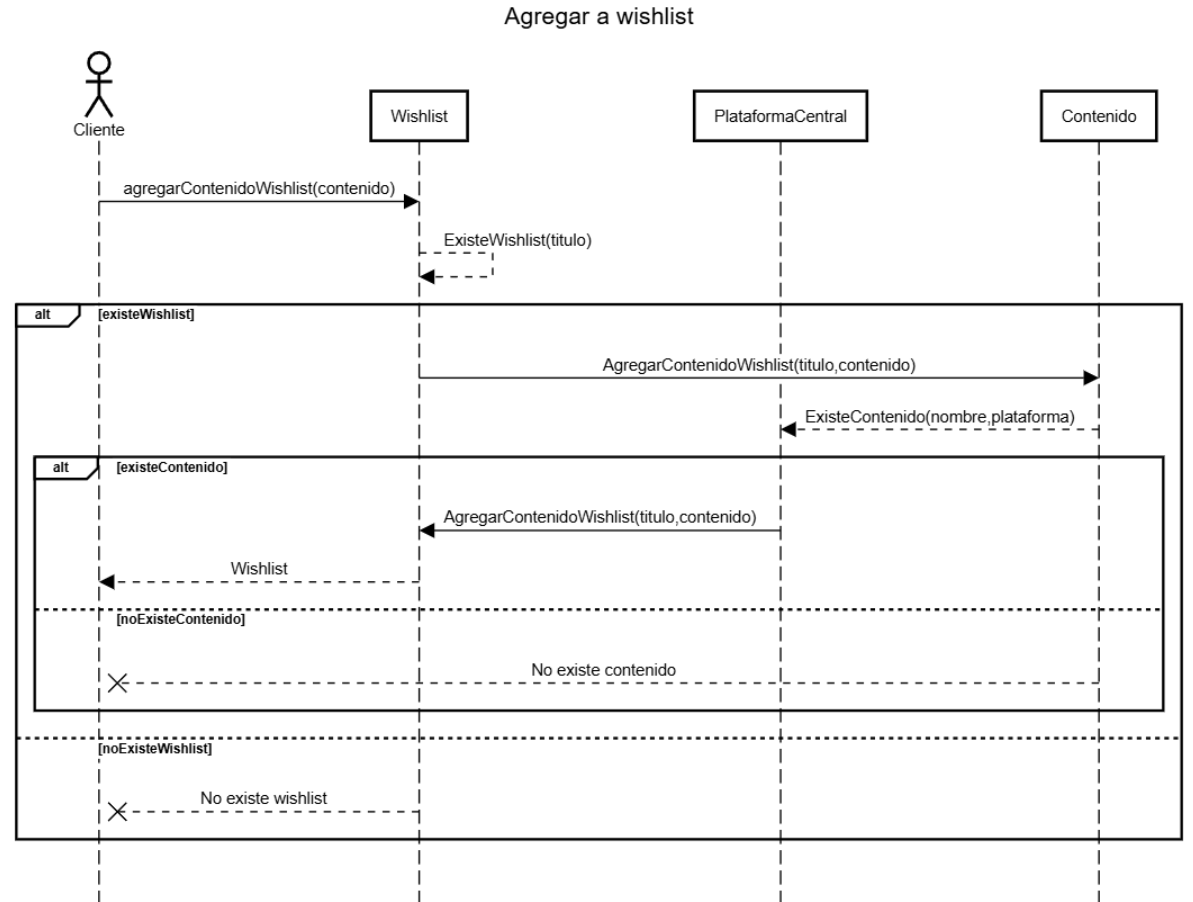
\includegraphics[width=1\textwidth]{img/agregar_a_wishlist}
\end{figure}

\clearpage

\subsection{Opinar y puntuar}\label{subsec:opinar-y-puntuar}
\begin{figure}[h]
    \centering
    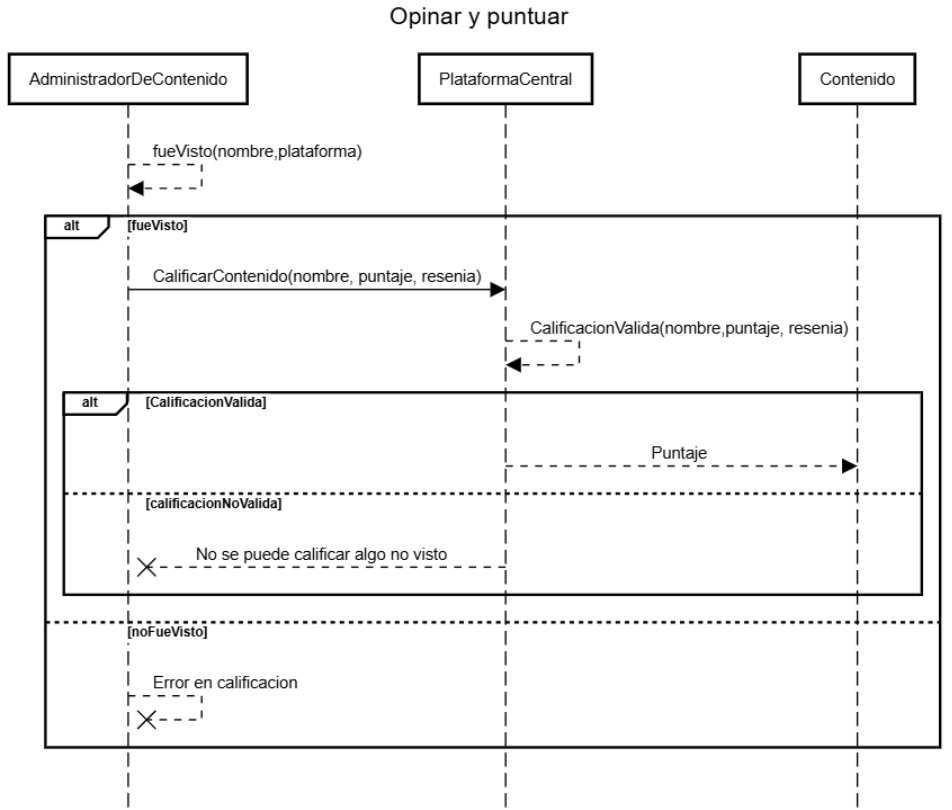
\includegraphics[width=0.8\textwidth]{img/opinar_y_puntuar}
\end{figure}

\subsection{Registrar cliente}\label{subsec:registrar-cliente}
\begin{figure}[h]
    \centering
    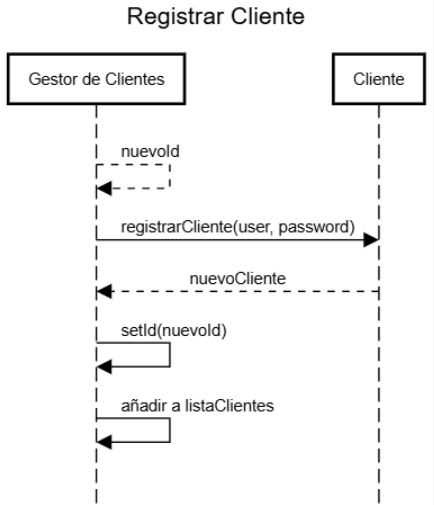
\includegraphics[width=0.4\textwidth]{img/registrar}
\end{figure}

\clearpage

\subsection{Últimos vistos}\label{subsec:ultimos-vistos}
\begin{figure}[h]
    \centering
    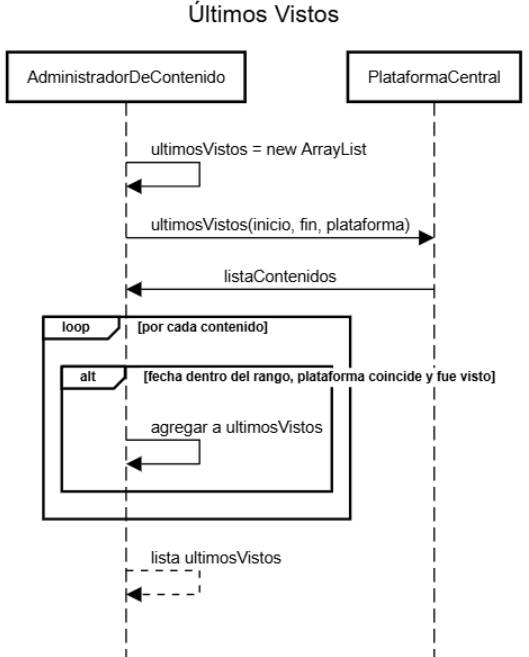
\includegraphics[width=0.9\textwidth]{img/ultimos_vistos}
\end{figure}

\clearpage

\subsection{Vistos}\label{subsec:vistos}
\begin{figure}[h]
    \centering
    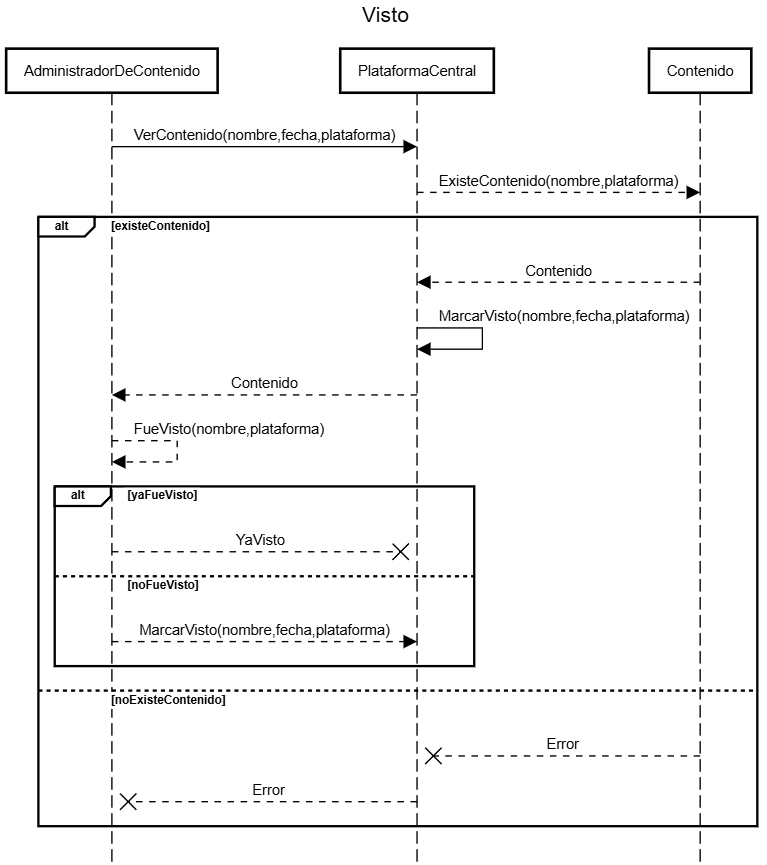
\includegraphics[width=1\textwidth]{img/visto}
\end{figure}

\clearpage

\section{Diagrama de clases}\label{sec:diagrama-de-clases}
\begin{figure}[h]
    \centering
    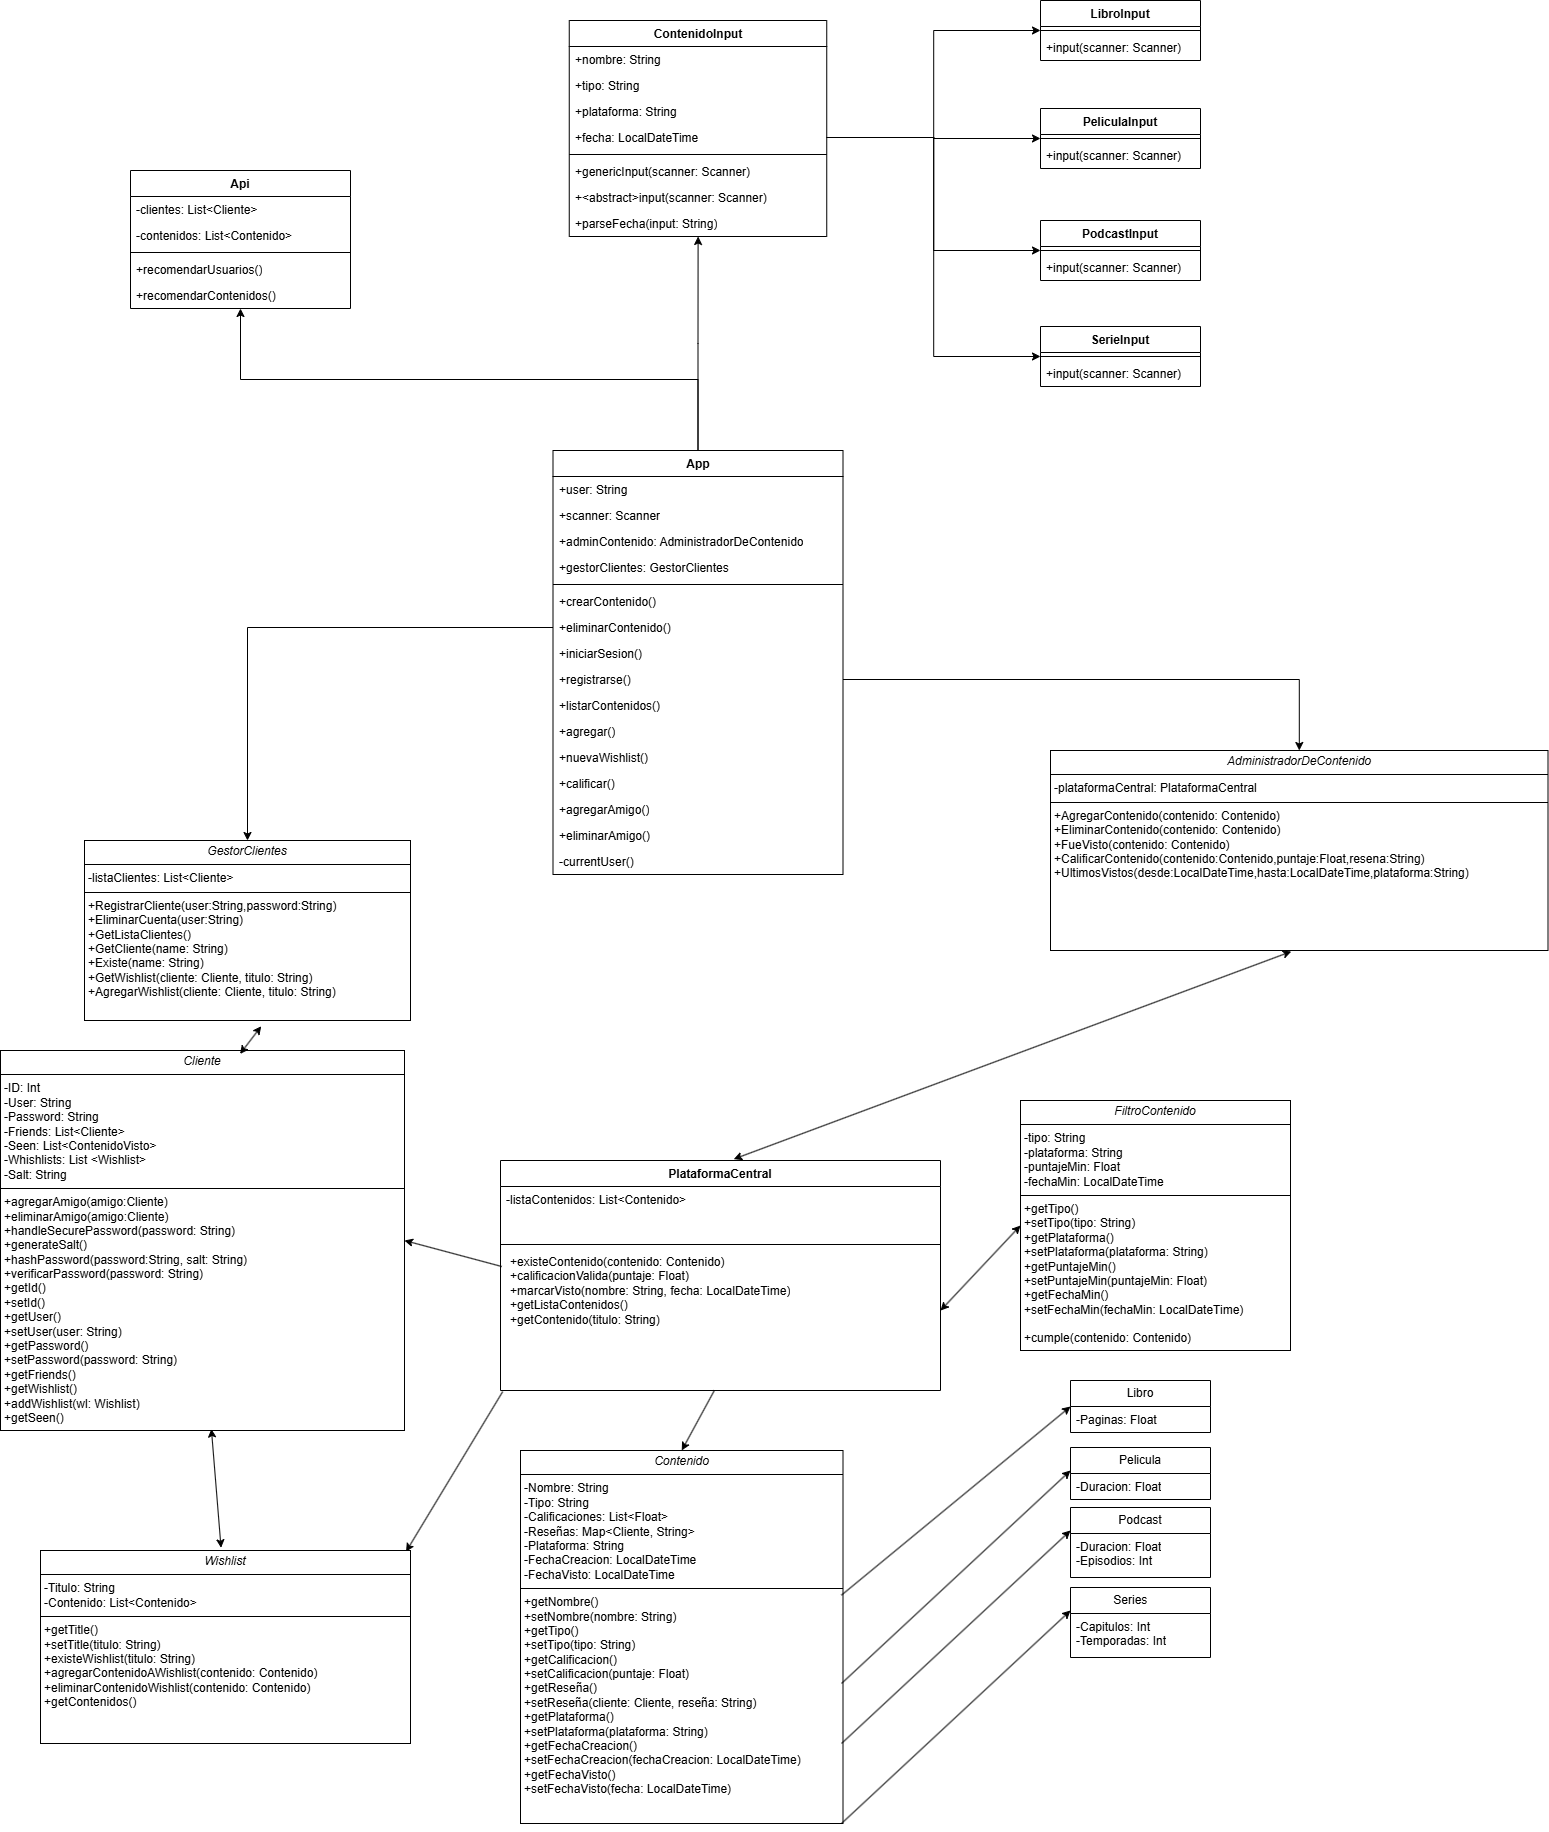
\includegraphics[width=1\textwidth]{img/diagrama_clases}
\end{figure}

    }

    \newpage
\end{document}
